\documentclass{article}

\usepackage{authblk} % for multiple authors and affiliations
\usepackage{graphicx} % to inlcude graphics with \includegraphics
\usepackage{tikz}
\usepackage{listings}
\usepackage{polyglossia}
\newfontfamily\nm{akaashnormal.ttf}
\usepackage[utf8]{inputenc}
\usepackage[T1]{fontenc}
\usepackage{fourier}

\usepackage{multirow}
%\usepackage{geometry}
\usepackage[utf8]{inputenc}
\usepackage{color}   %May be necessary if you want to color links
\usepackage{hyperref}
\hypersetup{
    colorlinks=true, %set true if you want colored links
    linktoc=all,     %set to all if you want both sections and subsections linked
    linkcolor=black,  %choose some color if you want links to stand out
}
% Please add the following required packages to your document preamble:
\usepackage{graphicx}
\usepackage[normalem]{ulem}
\useunder{\uline}{\ul}{}
% \usepackage[normalem]{ulem}
% \useunder{\uline}{\ul}{}
 \usepackage{longtable}

%New colors defined below
\definecolor{codegreen}{rgb}{0,0.6,0}
\definecolor{codegray}{rgb}{0.5,0.5,0.5}
\definecolor{codepurple}{rgb}{0.58,0,0.82}
\definecolor{backcolour}{rgb}{0.95,0.95,0.92}

%Code listing style named "mystyle"
\lstdefinestyle{mystyle}{
  backgroundcolor=\color{backcolour}, commentstyle=\color{codegreen},
  keywordstyle=\color{magenta},
  numberstyle=\tiny\color{codegray},
  stringstyle=\color{codepurple},
  basicstyle=\ttfamily\footnotesize,
  breakatwhitespace=false,         
  breaklines=true,                 
  captionpos=b,                    
  keepspaces=true,                 
  numbers=left,                    
  numbersep=5pt,                  
  showspaces=false,                
  showstringspaces=false,
  showtabs=false,                  
  tabsize=2
}

%"mystyle" code listing set
\lstset{style=mystyle}

\author{\textbf{PERPENDICOOLER}}
\date{}







\title{\textbf {Code for Numerical Analysis Executed in FORTRAN }}
%\affil{Department of Mathematics, Shahjalal University of Science and Technology, Sylhet, Bangladesh.}


\begin{document}


\maketitle

\section*{Abstract}
Fortran is a programming language that is well-suited for numerical analysis. It is a compiled language, which means that the code is converted into machine code before it is executed. This makes Fortran programs faster than interpreted languages, such as Python. Fortran also has a rich set of mathematical functions, which makes it easy to implement numerical algorithms.As a compiler, we used codeblocks 20.03.
\section*{Introduction}
Numerical analysis is the study of algorithms that use numerical approximation (as opposed to symbolic manipulations) for the problems of mathematical analysis (as distinguished from discrete mathematics). It is the study of numerical methods that attempt at finding approximate solutions of problems rather than the exact ones. Numerical analysis finds application in all fields of engineering and the physical sciences, and in the 21st century also the life and social sciences, medicine, business and even the arts. Current growth in computing power has enabled the use of more complex numerical analysis, providing detailed and realistic mathematical models in science and engineering. Examples of numerical analysis include: ordinary differential equations as found in celestial mechanics (predicting the motions of planets, stars and galaxies), numerical linear algebra in data analysis,and stochastic differential equations and Markov chains for simulating living cells in medicine and biology.
Fortran was originally developed in the 1950s for scientific and engineering applications. It was one of the first high-level programming languages, and it quickly became popular for numerical analysis. Fortran is still a popular language for numerical analysis today, and it is used by many scientists and engineers around the world.
\newpage
\tableofcontents
\newpage
\section{Root Finding}
In mathematics and computing, a root-finding algorithm is an algorithm for finding zeros, also called "roots", of continuous functions. A zero of a function f, from the real numbers to real numbers or from the complex numbers to the complex numbers, is a number x such that f(x) = 0. As, generally, the zeros of a function cannot be computed exactly nor expressed in closed form, root-finding algorithms provide approximations to zeros, expressed either as floating-point numbers or as small isolating intervals, or disks for complex roots (an interval or disk output being equivalent to an approximate output together with an error bound). \cite{press1992root}
Solving an equation f(x) = g(x) is the same as finding the roots of the function h(x) = f(x) – g(x). Thus root-finding algorithms allow solving any equation defined by continuous functions. However, most root-finding algorithms do not guarantee that they will find all the roots; in particular, if such an algorithm does not find any root, that does not mean that no root exists.\cite{press1992root}

Most numerical root-finding methods use iteration, producing a sequence of numbers that hopefully converges towards the root as its limit. They require one or more initial guesses of the root as starting values, then each iteration of the algorithm produces a successively more accurate approximation to the root. Since the iteration must be stopped at some point, these methods produce an approximation to the root, not an exact solution. Many methods compute subsequent values by evaluating an auxiliary function on the preceding values. The limit is thus a fixed point of the auxiliary function, which is chosen for having the roots of the original equation as fixed points, and for converging rapidly to these fixed points.

The behavior of general root-finding algorithms is studied in numerical analysis. However, for polynomials, root-finding study belongs generally to computer algebra, since algebraic properties of polynomials are fundamental for the most efficient algorithms. The efficiency of an algorithm may depend dramatically on the characteristics of the given functions. For example, many algorithms use the derivative of the input function, while others work on every continuous function. In general, numerical algorithms are not guaranteed to find all the roots of a function, so failing to find a root does not prove that there is no root. However, for polynomials, there are specific algorithms that use algebraic properties for certifying that no root is missed, and locating the roots in separate intervals (or disks for complex roots) that are small enough to ensure the convergence of numerical methods (typically Newton's method) to the unique root so located.
\begin{center}
    \begin{itemize}
        \item Bracketing methods
        \item Fixed point iteration method
    \end{itemize}
\end{center}
\newpage
\subsection{Bracketing Method}
Bracketing methods determine successively smaller intervals (brackets) that contain a root. When the interval is small enough, then a root has been found. They generally use the intermediate value theorem, which asserts that if a continuous function has values of opposite signs at the end points of an interval, then the function has at least one root in the interval. Therefore, they require to start with an interval such that the function takes opposite signs at the end points of the interval. However, in the case of polynomials there are other methods (Descartes' rule of signs, Budan's theorem and Sturm's theorem) for getting information on the number of roots in an interval. They lead to efficient algorithms for real-root isolation of polynomials, which ensure finding all real roots with a guaranteed accuracy.
\begin{center}
    \begin{itemize}
        \item Bisection
        \item Regula Falsi Method
    \end{itemize}
\end{center}
\subsubsection{Bisection Method}
The simplest root-finding algorithm is the bisection method. Let f be a continuous function, for which one knows an interval [a, b] such that f(a) and f(b) have opposite signs (a bracket). Let c = (a +b)/2 be the middle of the interval (the midpoint or the point that bisects the interval). Then either f(a) and f(c), or f(c) and f(b) have opposite signs, and one has divided by two the size of the interval. Although the bisection method is robust, it gains one and only one bit of accuracy with each iteration. Therefore, the number of function evaluations required for finding an $\epsilon$-approximate root is $ln \frac{b-a}{\epsilon}$
 Other methods, under appropriate conditions, can gain accuracy faster.
\subsubsection{Source Code}
\begin{lstlisting}[language=Fortran,caption=Bisection Method]
PROGRAM bisection
    IMPLICIT NONE
    REAL :: a,b,tol,er,p,f
    INTEGER :: i=1
    WRITE (*,*) "Enter [a,b] of the given equation"!--Take 0 and 1 as a interval--!
    READ (*,*) a,b
    WRITE (*,*) "The tolerance up to"
    READ (*,*) tol
    IF ((f(a)*f(b))== 0) THEN
        IF ((f(a)==0).and.(f(b)==0)) THEN
            WRITE (*,*) 'The roots are',a,' and ',b
        ELSE IF (f(a)==0) THEN
            WRITE (*,*) 'The root is',a
        ELSE IF (f(b)==0) THEN
            WRITE (*,*) 'The root is',b
        END IF
    ELSE IF ((f(a)*f(b))>0) THEN
        WRITE (*,*) 'The root does not exist in  ',a,' and ',b
    ELSE IF ((f(a)*f(b))<0) THEN
        open(10,file="output.txt")!--Here it will open a file named output.txt--!
        DO
            p=(a+b)/2
            IF (f(p)==0) EXIT
            er=abs((a-b)/a)
            WRITE (10,*) "Total Steps =",i,"The root is",p
            IF (er<((tol))) EXIT
            IF ((f(p)*f(a))<0) THEN

                b=p
            ELSE IF ((f(p)*f(b))<0) THEN
                a=p

            END IF
            i = i + 1
        END DO
    END IF

END PROGRAM

REAL FUNCTION f(x)
    f=x*exp(x)-1
END FUNCTION f
\end{lstlisting}
\begin{lstlisting}[language=Fortran,caption=Bisection Method Output]
 Total Steps =           1 The root is  0.500000000    
 Total Steps =           2 The root is  0.750000000    
 Total Steps =           3 The root is  0.625000000    
 Total Steps =           4 The root is  0.562500000    
 Total Steps =           5 The root is  0.593750000    
 Total Steps =           6 The root is  0.578125000    
 Total Steps =           7 The root is  0.570312500    
 Total Steps =           8 The root is  0.566406250    
 Total Steps =           9 The root is  0.568359375    
 Total Steps =          10 The root is  0.567382812    
 Total Steps =          11 The root is  0.566894531    
 Total Steps =          12 The root is  0.567138672    
 Total Steps =          13 The root is  0.567260742    
 Total Steps =          14 The root is  0.567199707    
 Total Steps =          15 The root is  0.567169189    
 Total Steps =          16 The root is  0.567153931    

\end{lstlisting}
\newpage
\subsubsection{Regula Falsi Method}
The false position method, also called the regula falsi method, is similar to the bisection method, but instead of using bisection search's middle of the interval it uses the x-intercept of the line that connects the plotted function values at the endpoints of the interval, that is $ c = \frac{a*f(b)-b*f(a)}{f(b)-f(a)}$
False position is similar to the secant method, except that, instead of retaining the last two points, it makes sure to keep one point on either side of the root. The false position method can be faster than the bisection method and will never diverge like the secant method; however, it may fail to converge in some naive implementations due to roundoff errors that may lead to a wrong sign for f(c); typically, this may occur if the rate of variation of f is large in the neighborhood of the root.
\subsubsection{Source Code}
\begin{lstlisting}[language=Fortran,caption=Regula Falsi]
PROGRAM regulafalsi
    REAL :: a,b,tol,p
    INTEGER :: i=1
   !!open(10,file="regulaFalsi.txt")!!--input from the file named regula falsi.txt--!!
    WRITE(*,*) "ENTER THE INTERVAL "
    READ (*,*) a,b!!--0 and 1 is the boundary value of this function where the root lies and tol is tolerance upto--!!
    WRITE(*,*)"ENTER THE TOLERANCE "
    READ(*,*)TOL
    open(11,file="regulaFalsioutput.txt")
    IF ((f(a)*f(b))>0) THEN
        WRITE (*,*) 'The root does not exist in  ',a,' and ',b
    ELSE IF ((f(a)*f(b))<0) THEN
        DO
            p=(a*f(b)-b*f(a))/(f(b)-f(a))
            IF (f(p)==0) EXIT

            WRITE (11,*) 'Total Steps =',i,'The root is',p
            IF (abs((a-b)/a)<((tol))) EXIT
                IF ((f(p)*f(a))<0) THEN

                b=p
                ELSE IF ((f(p)*f(b))<0) THEN
                a=p
            END IF
            i = i + 1
        END DO

   END IF

END PROGRAM

REAL FUNCTION f(x)
    f=x*exp(x)-2
END FUNCTION f




\end{lstlisting}
\begin{lstlisting}[language=Fortran,caption=Bisection Method Output]
 Total Steps =           1 The root is  0.735758901    
 Total Steps =           2 The root is  0.839520812    
 Total Steps =           3 The root is  0.851183891    
 Total Steps =           4 The root is  0.852451563    
 Total Steps =           5 The root is  0.852588832    
 Total Steps =           6 The root is  0.852603674    
 Total Steps =           7 The root is  0.852605283    
 Total Steps =           8 The root is  0.852605402    
 Total Steps =           9 The root is  0.852605462    
 

\end{lstlisting}

\subsection{Fixed Point Method}
Although all root-finding algorithms proceed by iteration, an iterative root-finding method generally uses a specific type of iteration, consisting of defining an auxiliary function, which is applied to the last computed approximations of a root for getting a new approximation. The iteration stops when a fixed point (up to the desired precision) of the auxiliary function is reached, that is when the new computed value is sufficiently close to the preceding ones.\\
\begin{center}
    \begin{itemize}
        \item Iterative Method .
        \item Newton-Rhapson Method .
    \end{itemize}
\end{center}
\subsubsection{Iterative Method}
We can use the fixed-point iteration to find the root of a function. Given a function $ f(x)$ which we have set to zero to find the root $f(x) = 0$we rewrite the equation in terms of $x$ so that $f(x) = 0$ becomes $x = g(x)$ (note, there are often many $g(x)$ functions for each $f(x) = 0$, function)/ Next, We relavel each side of the equation as $x_{n+1} \ =\ g( x_{n})$o that we can perform the iteration. Next, we pick a value for $x_1$ and perform the iteration until it converges towards a root of the function. If the iteration converges, it will converge to a root. The iteration will only converge if $|g'( root) |< 1$ \
As an example of converting $f(x) = 0 $ to $ x = g(x) $, if given finciton $f(x) = x^2+x-1$ , We will rewrite it as one of the following equations \\
$
x_{n+1} \ =\ \frac{1}{x_{n}} -1\ ,\\
x_{n+1} \ =\frac{1}{x_{n} +1} \ ,\\
x_{n+1} \ =1-x_{n}^{2} \ ,\\
x_{n+1} \ =x_{n}^{2} +2x_{n} -1\ ,\ \\
x_{n+1} \ =\pm \sqrt{1-x_{n}} .
$

\subsubsection{Source Code}
\begin{lstlisting}[language=Fortran,caption=Iterative Method]
program iteration

    real :: x,x0,e
    integer :: i=1,n
    !open(10,file='iterationMethod.txt')
    open(11,file='iterationMethodOutput.txt')
    write(*,*)"Enter the initial guess."
    read(*,*)x0!!--x0 is initial guess,n is number of steps and e is tolerance up to--!!
    write(*,*)"Enter the tolerance"
    read(*,*)e!!--0.0001--!

    do
        x=g(x0)
        write(11,*)"number of steps = ",i," The root x is : ",x
        IF (abs(x-x0)<=e) EXIT
        x0=x
        i=i+1
    end do

end program

real function f(x)
    real :: x
    f=x*exp(x)-1
    return
end function

real function g(x)
    real :: x
    g=exp(-x)
    return
end function





\end{lstlisting}
\begin{lstlisting}[language=Fortran,caption=Iterative Method Output]
 number of steps =            1  The root x is :   0.367879450    
 number of steps =            2  The root x is :   0.692200601    
 number of steps =            3  The root x is :   0.500473499    
 number of steps =            4  The root x is :   0.606243551    
 number of steps =            5  The root x is :   0.545395792    
 number of steps =            6  The root x is :   0.579612315    
 number of steps =            7  The root x is :   0.560115457    
 number of steps =            8  The root x is :   0.571143091    
 number of steps =            9  The root x is :   0.564879358    
 number of steps =           10  The root x is :   0.568428695    
 number of steps =           11  The root x is :   0.566414773    
 number of steps =           12  The root x is :   0.567556620    
 number of steps =           13  The root x is :   0.566908896    
 number of steps =           14  The root x is :   0.567276239    
 number of steps =           15  The root x is :   0.567067921    
 number of steps =           16  The root x is :   0.567186058    
 number of steps =           17  The root x is :   0.567119062    
 
\end{lstlisting}
\newpage
\subsubsection{Newton Raphson Method}
The Newton-Raphson method (also known as Newton's method) is a way to quickly find a good approximation for the root of a real-valued function \(f(x) = 0\). It uses the idea that a continuous and differentiable function can be approximated by a straight line tangent to it.

Suppose you need to find the root of a continuous, differentiable function \(f(x)\), and you know the root you are looking for is near the point \(x = x_0\). Then Newton's method tells us that a better approximation for the root is \[x_1 = x_0 - \frac{f(x_0)}{f'(x_0)}.\] This process may be repeated as many times as necessary to get the desired accuracy. In general, for any \(x\)-value \(x_n\), the next value is given by \[x_{n+1} = x_n - \frac{f(x_n)}{f'(x_n)}.\]

Note: the term "near" is used loosely because it does not need a precise definition in this context. However, \(x_0\) should be closer to the root you need than to any other root (if the function has multiple roots).\newline
Here is a picture to demonstrate what Newton's method actually does:\newline
\begin{center}
    \begin{figure}[h!]
        \centering
        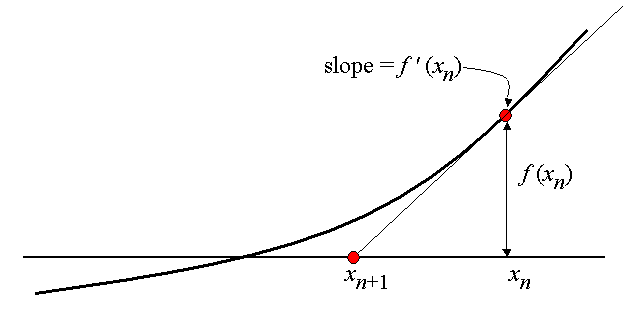
\includegraphics[width=8cm]{7KrMvNiT7l-newtons-method.png}
        \caption{Caption}
        \label{fig:enter-label}
    \end{figure}
\end{center}
We draw a tangent line to the graph of \(f(x)\) at the point \(x = x_n\). This line has slope \(f'(x_n)\) and goes through the point \(\big(x_n, f(x_n)\big)\). Therefore it has the equation \(y = f'(x_n)(x - x_n) + f(x_n)\). Now, we find the root of this tangent line by setting \(y = 0\) and \(x=x_{n+1}\) for our new approximation. Solving this equation gives us our new approximation, which is \(x_{n+1} = x_n - \frac{f(x_n)}{f'(x_n)}\).
\newline
Find the root of the equation \(x^2 - 4x - 7 = 0\) near \(x = 5\) to the nearest thousandth.

We have our \(x_0 = 5\). In order to use Newton's method, we also need to know the derivative of \(f\). In this case, \(f(x) = x^2 - 4x - 7\), and \(f'(x) = 2x - 4\).

Using Newton's method, we get the following sequence of approximations:

$ x_1 = 5 - \frac{5^2 - 4\times 5 - 7}{2\times 5 - 4} = 5 - \left(\frac{-2}{6}\right) = \frac{16}{3} \approx 5.33333\\ x_2 = \frac{16}{3} - \frac{\left(\frac{16}{3}\right)^2 - 4\left(\frac{16}{3}\right) - 7}{2\left(\frac{16}{3}\right)-4} = \frac{16}{3} - \frac{\frac{1}{9}}{\frac{20}{3}} = \frac{16}{3} - \frac{1}{60} = \frac{319}{60} \approx 5.31667 \\ x_3 = \frac{319}{60} - \frac{\left(\frac{319}{60}\right)^2 - 4\left(\frac{319}{60}\right) - 7}{2\left(\frac{319}{60}\right)-4} = \frac{319}{60} - \frac{\frac{1}{3600}}{\frac{398}{60}} \approx 5.31662.$  

We can stop now, because the thousandth and ten-thousandth digits of \(x_2\) and \(x_3\) are the same. If we were to continue, they would remain the same because we have gotten sufficiently close to the root:

\[x_4 = 5.31662 - \frac{(5.3362)^2-4(5.3362)-7}{2(5.3362)-4} = 5.31662.\]

Our final answer is therefore 5.317. \( _\square \)\cite{newtonraphson}
\subsubsection{Source Code}
\begin{lstlisting}[language=Fortran,caption=Newton Raphson Method]
program newtonRaphson
    integer::i=1
    real::x,x0,e
    !open(10,file="nr.txt")!!--Reading the file from the file nr.txt--!!
    open(11,file="nroutput.txt")
    WRITE(*,*)"Enter the initial guess"
    READ(*,*)x0!!--x0=2 is initial guess,e is tolerance up to--!!
    WRITE(*,*)"Enter the tolerance"!!--0.0001--!
    read(*,*)e

    do
        x=x0-(f(x0)/df(x0))
        write(11,*)"Number of steps ",i, " the root x is =",x
        IF (ABS(x-x0)<=e) EXIT
        x0=x
        i=i+1
    end DO

 end program

 real function f(x)
    real::x
    f=x**3-2*x-5
    return
 end

real function df(x)
    real::x
    df=3*x**2-2
    return
end





\end{lstlisting}
\begin{lstlisting}[language=Fortran,caption=Newton Rhapson Method Output]
 Number of steps            1  the root x is =   2.09999990    
 Number of steps            2  the root x is =   2.09456801    
 Number of steps            3  the root x is =   2.09455156    
\end{lstlisting}
\section{Interpolation And Extrapolation}
\subsection{Finite Difference}
\subsubsection{Finite Forward Difference}
\begin{center}
\begin{tabular}{ |c|c|c| } 
\hline
 x & y\\
 \hline
 45 & 2.871  \\  \hline
 50 & 2.404  \\  \hline
 55 & 2.083 \\  \hline
 60 & 1.862  \\  \hline
 65 & 1.712 \\  \hline
 
 \hline
\end{tabular}
\end{center}
\subsubsection{Source Code}
Data Value in file given as below\\
5\\
45\\
2.871\\
50\\
2.404\\
55\\
2.083\\
60\\
1.862\\
65\\
1.712\\


\begin{lstlisting}[language=Fortran,caption=Finite Forward Difference]
program finiteForwardDifference
    real x(10),y(10,10)
    real i,j,n
    print*,'enter number of data'

    open(10,file="data.txt")!!--The data will read from the file named data--!!
    read(10,*),n
    do i=1,n
        !print*,'X[',i,']='
        read(10,*),x(i)
        !print*,'y[',i,']='
        read(10,*),y(i,1)
    end do
    do j=2,n
        do i=1,n-j+1
            y(i,j)=y(i+1,j-1)-y(i,j-1)
        end do
    end do
    print*,'Forward difference table:'
    do i=1,n
        print"(10f10.3)",x(i),(y(i,j),j=1,n-i+1)

    end do

end program






\end{lstlisting}
\begin{lstlisting}[language=Fortran,caption=Finite Forward Difference Output]
 Forward difference table:
    45.000     2.871    -0.467     0.146    -0.046     0.017
    50.000     2.404    -0.321     0.100    -0.029
    55.000     2.083    -0.221     0.071
    60.000     1.862    -0.150
    65.000     1.712

Process returned 0 (0x0)   execution time : 0.032 s
Press any key to continue.
 
\end{lstlisting}
\subsubsection{Finite Backward Difference}
\begin{center}
\begin{tabular}{ |c|c|c| } 
\hline
 x & y\\
\hline
 1 & 1  \\  \hline
 2 & 8  \\  \hline
 3 & 27 \\  \hline
 4 & 64  \\  \hline
 5 & 125  \\  \hline
 
 \hline
\end{tabular}
\end{center}
\subsubsection{Source Code}
Data Value in file given as below\\
5\\
1\\
1\\
2\\
8\\
3\\
27\\
4\\
64\\
5\\
125\\





\begin{lstlisting}[language=Fortran,caption=Finite Backward Difference]
program finiteBackwardDifference
    real x(10),y(10,10)
    real i,j,n
   !print*,'enter number of data'

    open(10,file="data2.txt")
    read(10,*),n
    do i=1,n
        !print*,'X[',i,']='
        read(10,*),x(i)
        !print*,'y[',i,']='
        read(10,*)y(i,1)
    end do
    do j=2,n
        do i=1,n-j+5
            y(i+1,j)=y(i+1,j-1)-y(i,j-1)
        end do
    end do
    print*,'Backward difference table:'
    do i=1,n
        print"(10f10.3)",x(i),(y(i,j),j=1,i)
    end do


end program






\end{lstlisting}
\begin{lstlisting}[language=Fortran,caption=Finite Backward Difference Output]
 Backward difference table:
       1.0       1.0
       2.0       8.0       7.0
       3.0      27.0      19.0      12.0
       4.0      64.0      37.0      18.0       6.0
       5.0     125.0      61.0      24.0       6.0       0.0

Process returned 0 (0x0)   execution time : 0.039 s
Press any key to continue.
\end{lstlisting}
\subsection{Newton Gregory Interpolation}
\subsubsection{Newton Forward Interpolation}
\begin{center}
\begin{tabular}{ |c|c|c| } 
\hline
 x & y\\
 \hline
 45 & 2.871  \\  \hline
 50 & 2.404  \\  \hline
 55 & 2.083 \\  \hline
 60 & 1.862  \\  \hline
 65 & 1.712 \\  \hline
 
 \hline
\end{tabular}
\end{center}
\subsubsection{Source Code}
Data Value in file given as below\\
5\\
45\\
2.871\\
50\\
2.404\\
55\\
2.083\\
60\\
1.862\\
65\\
1.712\\
Find the value on $f(46)$.


\begin{lstlisting}[language=Fortran,caption=Newton Forward Interpolation]
program newtonForwardInterpolation
    real x(10),y(10,10)
    real i,j,n,p,h,u,poly,ut,fact!!--poly is declared for the total functioanl value --!!
    !print*,'enter number of data'

    open(10,file="data.txt")
    read(10,*),n
    do i=1,n
        !print*,'X[',i,']='
        read(10,*),x(i)
        !print*,'y[',i,']='
        read(10,*),y(i,1)
    end do
    do j=2,n
        do i=1,n-j+1
            y(i,j)=y(i+1,j-1)-y(i,j-1)
        end do
    end do
    print*,'Forward difference table:'
    do i=1,n
        print"(10f10.3)",x(i),(y(i,j),j=1,n-i+1)

    end do
    print*,"Enter the data value you want"!!--for ex enter 46 --!
    read*,p
    h=x(2)-x(1)
    print*,"The gap between two number",h
    u=(p-x(1))/h
    ut=u
    poly=y(1,1)
    fact=1
    do i=2,n
        poly=poly+ut*y(1,i)/fact
        fact=fact*i
        ut=ut*(u-(i-1))
    end do
    print*,"The functional value of the demand value is",poly
end program


\end{lstlisting}
\begin{lstlisting}[language=Fortran,caption=Newton Forward Interpolation Output]
 Forward difference table:
    45.000     2.871    -0.467     0.146    -0.046     0.017
    50.000     2.404    -0.321     0.100    -0.029
    55.000     2.083    -0.221     0.071
    60.000     1.862    -0.150
    65.000     1.712
 Enter the data value you want
46
 The gap between two number   5.00000000
 The functional value of the demand value is   2.76314092

Process returned 0 (0x0)   execution time : 2.682 s
Press any key to continue.

\end{lstlisting}
\subsubsection{Newton Backward Interpolation}
\begin{center}
\begin{tabular}{ |c|c|c| } 
\hline
 x & y\\
\hline
 1 & 1  \\  \hline
 2 & 8  \\  \hline
 3 & 27 \\  \hline
 4 & 64  \\  \hline
 5 & 125  \\  \hline

 
 \hline
\end{tabular}
\end{center}
\subsubsection{Source Code}
Data Value in file given as below\\
5\\
1\\
1\\
2\\
8\\
3\\
27\\
4\\
64\\
5\\
125\\
Find the value on $f(3.5)$\\





\begin{lstlisting}[language=Fortran,caption=Newton Backward Interpolation]
program newtonBackwardInterpolation
    real x(10),y(10,10)
    real i,j,n,p,h,v,poly,vt,factfun
    !print*,'enter number of data'

    open(10,file="data2.txt")
    read(10,*),n
    do i=1,n
        !print*,'X[',i,']='
        read(10,*),x(i)
        !print*,'y[',i,']='
        read(10,*)y(i,1)
    end do
    do j=2,n
        do i=1,n-j+5
            y(i+1,j)=y(i+1,j-1)-y(i,j-1)
        end do
    end do
    print*,'Backward difference table:'
    do i=1,n
        print"(10f10.3)",x(i),(y(i,j),j=1,i)
    end do
    print*,"Enter the data value you want"
    read*,p
    h=x(2)-x(1)
    print*,"The gap between two number",h
    v=(p-x(n))/h
!   print*,"the value of y(1,2)",y(1,2)
    vt=v
    print*,"the value of v is",v
    poly=y(n,1)
    !print*,"the value stored in poly",poly
    fact=1
    do i=2,n
        poly=poly+vt*y(n,i)/fact
        fact=fact*i
        vt=vt*(v+(i-1))
    end do
    print*,"The functional value of the demand value is",poly
end program








\end{lstlisting}
\begin{lstlisting}[language=Fortran,caption=Newton Backward Interpolation Output]
 Backward difference table:
     1.000     1.000
     2.000     8.000     7.000
     3.000    27.000    19.000    12.000
     4.000    64.000    37.000    18.000     6.000
     5.000   125.000    61.000    24.000     6.000     0.000
 Enter the data value you want
3.5
 The gap between two number   1.00000000
 the value of v is  -1.50000000
 The functional value of the demand value is   42.8750000

Process returned 0 (0x0)   execution time : 1.260 s
Press any key to continue.
\end{lstlisting}
\subsection{Newton Divided Interpolation}
\begin{center}
\begin{tabular}{ |c|c|c| } 
\hline
 x & y\\
 \hline
 4 & 48  \\  \hline
 5 & 100  \\  \hline
 7 & 294 \\  \hline
 10 & 900  \\  \hline
 11 & 1210  \\  \hline
 13 & 2028 \\ \hline

 
 \hline
\end{tabular}
\end{center}
\subsubsection{Source Code}
Data Value in file given as below\\
6\\
4\\
48\\
5\\
100\\
7\\
294\\
10\\
900\\
11\\
1210\\
13\\
2028\\
Find the value on $f(8)$\\





\begin{lstlisting}[language=Fortran,caption=Newton Divided Interpolation]
program newtonDividedInterpolation
    real x(10),y(10,10)
    real i,j,n,f,poly
    !print*,'enter number of data'

    open(10,file="input.txt")
    read(10,*),n
    do i=1,n
        !print*,'X[',i,']='
        read(10,*),x(i)
        !print*,'y[',i,']='
        read(10,*),y(i,1)
    end do
    do j=2,n
        do i=1,n-j+1
            y(i,j)=(y(i+1,j-1)-y(i,j-1))/(x(i+j-1)-x(i))
        end do
    end do
    print*,'Divided difference table:'
    do i=1,n
        print"(10f10.1)",x(i),(y(i,j),j=1,n-i+1)
    end do
    print*,"Enter the data value you want"!!--f(8)--so enter 8 to get the answer 448--!
    read*,f
    poly=y(1,1)
    !print*,"the value stored in poly",poly
    DO i=1,n-1
        p=1.0
            DO j=1,i
                p=p*(f-x(j))
            END DO
        poly=poly+p*y(1,i+1)
    END DO
    print"(A,F7.1)","The functional value of the demand value is",poly
end program












\end{lstlisting}
\begin{lstlisting}[language=Fortran,caption=Newton Divided Interpolation Output]
 Divided difference table:
    4.0      48.0      52.0      15.0       1.0       0.0       0.0
    5.0     100.0      97.0      21.0       1.0       0.0
    7.0     294.0     202.0      27.0       1.0
    10.0     900.0     310.0      33.0
    11.0    1210.0     409.0
    13.0    2028.0
 Enter the data value you want
8
The functional value of the demand value is  448.0

Process returned 0 (0x0)   execution time : 1.527 s
Press any key to continue.
\end{lstlisting}
\subsection{Lagrange Polynomial}
The Lagrange interpolation formula is a way to find a polynomial which takes on certain values at arbitrary points. Specifically, it gives a constructive proof of the theorem below.
\newline
Suppose we have one point (1,3). How can we find a polynomial that could represent it? \[ P(x) = 3 \] \[ P(1) = 3 \]\newline
Suppose we have sequence of points: (1,3), (2,4). How can we find a polynomial that could represent it? \[ P(x) = \frac {(x - 2)}{(1-2)} \times 3 + \frac {(x - 1)}{(2-1)} \times 4 \] \[P(1) = 3\\P(2) = 4 \]\\
Suppose we have sequence of points: (1,3), (2,4), (7,11). How can we find a polynomial that could represent it? \[ P(x) = \frac {(x-2)(x-7)}{(1-2)(1-7)} \times 3 + \frac {(x-1)(x-7)}{(2-1)(2-7)} \times 4 + \frac {(x-1)(x-2)}{(7-1)(7-2)} \times 11 \] \[P(1) = 3\\P(2) = 4\\P(7) = 11 \] In a general form it looks like this: \[ P ( x ) = \frac { \left( x - x _ { 2 } \right) \left( x - x _ { 3 } \right) } { \left( x _ { 1 } - x _ { 2 } \right) \left( x _ { 1 } - x _ { 3 } \right) } y _ { 1 } + \frac { \left( x - x _ { 1 } \right) \left( x - x _ { 3 } \right) } { \left( x _ { 2 } - x _ { 1 } \right) \left( x _ { 2 } - x _ { 3 } \right) } y _ { 2 } + \frac { \left( x - x _ { 1 } \right) \left( x - x _ { 2 } \right) } { \left( x _ { 3 } - x _ { 1 } \right) \left( x _ { 3 } - x _ { 2 } \right) } y _ { 3 } \] \[ P(x) = \sum _1^3 P_i (x) y_i \]\\ 
Given \( n \) distinct real values \( x_1, x_2, \ldots, x_n \) and \( n \) real values \( y_1, y_2, \ldots, y_n\) (not necessarily distinct), there is a unique polynomial \(P\) with real coefficients satisfying \( P(x_i)=y_i\) for \( i \in \{ 1,2, \ldots, n \} \), such that \( \text{deg}(P) < n.\) \(_\square\)\\
This theorem can be viewed as a generalization of the well-known fact that two points uniquely determine a straight line, three points uniquely determine the graph of a quadratic polynomial, four points uniquely determine the graph of a cubic polynomial, and so on. (Two caveats: (1) the points are required to have different \(x\)-coordinates, and (2) the "quadratic polynomial" might actually be a linear or constant polynomial, the "cubic polynomial" might actually be a quadratic, linear, or constant polynomial, and so on.)\\
First, a proof that the polynomial \( P \) is unique: Suppose \( Q\) and \( R\) are polynomials with the above properties. Then \( Q-R\) vanishes on \( x_1,x_2,\ldots,x_n,\) but its degree is less than \( n.\) A nonzero polynomial of degree \( <n\) cannot have \(n\) roots, so \( Q-R\) must be the zero polynomial, i.e. \( Q=R.\)

Now, to show that \( P\) exists, let \[ P_1(x) = \frac{(x-x_2)(x-x_3)(\cdots)(x-x_n)}{(x_1-x_2)(x_1-x_3)(\cdots)(x_1-x_n)}. \] Then \( P_1(x_1)=1 \) and \( P_1(x_2)=P_1(x_3)=\cdots=P_1(x_n)=0.\)

Similarly construct polynomials \( P_2,P_3,\ldots,P_n\) such that \( P_j (x_j)=1\) and \( P_j (x_i)=0\) for all \( i \neq j\). (One way to write \(P_j(x)\) is \[ P_j(x) = \frac{f(x)}{(x-x_j)f'(x_j)}, \] where \( f(x) = (x-x_1)(x-x_2)(\cdots)(x-x_n).)\)

Then, \( P(x) = \sum y_i P_i(x) \) is a polynomial with real coefficients satisfying \( P(x_i)=y_i\) for all \( i \in \{ 1,2, \ldots n \} \). It is a sum of polynomials of degree \( n-1,\) so its degree is \( <n.\) \(_\square\)\\
Using Lagrange interpolation to find a polynomial \(P\) of degree \( <4\) satisfying

$ P(1)=1, P(2)=4, P(3)=1, P(4)=5,$

what are the polynomials \( P_1(x), P_2(x), P_3(x), P_4(x), P(x)\)?

Let \( f(x) = (x-2)(x-3)(x-4)\). Then \[ f(1) = (-1)(-2)(-3)=-6 \text{, so } P_1(x) = -\frac {1}{6}(x-2)(x-3)(x-4).\]

Let $ f(x) = (x-1)(x-3)(x-4).$ $Then  f(2) = (1)(-1)(-2) = 2 \text{, so } P_2 (x) = \frac {1}{2} (x-1)(x-3)(x-4) $

Let \( f(x) = (x-1)(x-2)(x-4)\). Then \[ f(3) = (2)(1)(-1) = -2 \text{, so } P_3 (x) = -\frac {1}{2} (x-1)(x-2)(x-4). \]

Let \( f(x) = (x-1)(x-2)(x-3)\). Then \[ f(4) = (3)(2)(1) = 6 \text{, so } P_4 (x) = \frac {1}{6} (x-1)(x-2)(x-3). \]

Hence, $\ P(x) = 1\times \left(-\frac {1}{6}\right)(x-2)(x-3)(x-4) + 4\times \frac {1}{2} (x-1)(x-3)(x-4)\\ + 1\times \left(-\frac {1}{2}\right) (x-1)(x-2)(x-4)+ 5 \times \frac {1}{6} (x-1)(x-2)(x-3). $
\newline

Simplifying gives \( P(x) = \frac{13}6 x^3 -16x^2+\frac{215}6 x -21.\) \(_\square\)
\newline

\large{Example table}
\begin{center}

\begin{tabular}{ |c|c|c| } 
\hline
 x & y\\
 \hline
 1 & 4  \\  \hline
 2 & 5  \\  \hline
 7 & 5 \\  \hline
 8 & 4  \\  \hline


 
 \hline
\end{tabular}
\end{center}
\subsubsection{Source Code}
Data Value in file given as below\\
4\\
1 \\
4 \\
2 \\
5 \\
7 \\
5\\
8 \\
4\\
Find the value on $f(6)$\\





\begin{lstlisting}[language=Fortran,caption=Lagrange Polynomial]
program lagrangian_polynomial
    real x(10),y(10),p,k,s
    integer i,j,n

!print *,'Number of terms?'
    open(10,file="lagrange_input.txt")
    read(10,*)n
    do i=1,n
        read(10,*),x(i)
        read(10,*),y(i)
    end do
    print*,"The given data values are:"
    do i=1,n
        print*," x ",i," = ",x(i)," y ",i,"=",y(i)

    end do
    print *,"enter the data point to calculate the value"
    READ(*,*)k!!--Enter the value 6 to get f(6)=5.66--!!

    do i=1,n
        p=1.0
        do j=1,n
            if(i .ne. j) then
            p=p*((k-x(j))/(x(i)-x(j)))
            end if
        end do
        s=s+(p*y(i))
    end do
print *,"the value of that point ",k ,"is",s

end program













\end{lstlisting}
\begin{lstlisting}[language=Fortran,caption=Lagrange Polynomial Output]
 The given data values are:
  x  1  =    1.00000000      y  1 =   4.00000000
  x  2  =    2.00000000      y  2 =   5.00000000
  x  3  =    7.00000000      y  3 =   5.00000000
  x  4  =    8.00000000      y  4 =   4.00000000
 enter the data point to calculate the value
6
 the value of that point    6.00000000     is   5.66666698

Process returned 0 (0x0)   execution time : 1.931 s
Press any key to continue.
\end{lstlisting}
\section{Numerical Differentiation}
\subsection{Derivative using Newton Forward Difference formula}
\begin{center}
\begin{tabular}{ |c|c|c| } 
\hline
 x & y\\
 \hline
 3.0 & -14.00  \\  \hline
 3.2 & -10.032  \\  \hline
 3.4 & -5.296 \\  \hline
 3.6 & 0.256  \\  \hline
 3.7 & 6.672 \\  \hline
 4.0 & 14.00\\ \hline
 
 \hline
\end{tabular}
\end{center}
\subsubsection{Source Code}
Data Value in file given as below\\
6\\
3\\
-14.00\\
3.2\\
-10.032\\
3.4\\
-5.296\\
3.6\\
0.256\\
3.8\\
6.672\\
4\\
14\\
Find the first and second derivative of the function tabulated below, at the point $x=3$.



\begin{lstlisting}[language=Fortran,caption=Numerical Forward Differentiation]
program forward_differentiation
    real x(10),y(10,10)
    real i,j,n,h,diff,sm,fact,p,term,second_diff
    !print*,'enter number of data'
    open(10,file="data.txt")
    read(10,*),n
    do i=1,n
        !print*,'X[',i,']='
        read(10,*),x(i)
        !print*,'y[',i,']='
        read(10,*),y(i,1)
    end do
    do j=2,n
        do i=1,n-j+1
            y(i,j)=y(i+1,j-1)-y(i,j-1)
        end do
    end do
    print*,'Forward difference table:'
    do i=1,n
        print"(10f10.3)",x(i),(y(i,j),j=1,n-i+1)
    end do
    fact=1
    sm=0
    h=x(2)-x(1)
    !sm=sm/h
    do i=1,n
        term=y(1,i+1)/i
        sm=sm+fact*term
        fact=-fact
    end do
    diff=sm/h
    do i=1,1
         second_diff=y(1,i+2)-y(1,i+3)+(11/12)*y(1,i+4)-(5/6)*y(1,i+5)
         second_diff=second_diff*(1/h**2)
    end do
    write(*,"(A,F6.2,1x,A,F6.2)")"The first derivative of tabulated value on",x(1),"is",diff
    write(*,"(A,F6.2,1x,A,F6.2)")"The second derivative of tabulated value on",x(1), "is",second_diff

end program







\end{lstlisting}
\begin{lstlisting}[language=Fortran,caption=Numerical Forward Differentiation Output]
 Forward difference table:
    3.000  -14.000    3.968   0.768    0.048   -0.000   0.000
    3.200  -10.032    4.736   0.816    0.048    0.000
    3.400   -5.296    5.552   0.864    0.048
    3.600    0.256    6.416   0.912
    3.800    6.672    7.328
    4.000   14.000
The first derivative of tabulated value on  3.00 is 18.00
The second derivative of tabulated value on  3.00 is 18.00

Process returned 0 (0x0)   execution time : 0.040 s
Press any key to continue.
 
\end{lstlisting}
\subsection{Derivative using Newton backward Difference formula}
\begin{center}
\begin{tabular}{ |c|c|c| } 
\hline
 x & y\\
 \hline
 1.4 & 4.0552  \\  \hline
 1.6 & 4.9530  \\  \hline
 1.8 & 6.0496 \\  \hline
 2.0 & 7.3891  \\  \hline
 2.2 & 9.0250 \\  \hline

 
 \hline
\end{tabular}
\end{center}
\subsubsection{Source Code}
Data Value in file given as below\\
5\\
1.4\\
4.0552\\
1.6\\
4.9530\\
1.8\\
6.0496\\
2.0\\
7.3891\\
2.2\\
9.0250\\
Find the first and second derivative of the function tabulated below, at the point $x=2.2$.



\begin{lstlisting}[language=Fortran,caption=Numerical Backward Differentiation]
program backward_differentiation
    real x(10),y(10,10)
    real i,j,n,h,diff,sm,fact,p,term,second_diff
    !print*,'enter number of data'
    open(10,file="data.txt")
    read(10,*),n
   do i=1,n
        !print*,'X[',i,']='
        read(10,*),x(i)
        !print*,'y[',i,']='
        read(10,*)y(i,1)
    end do
    do j=2,n
        do i=1,n-j+10
            y(i+1,j)=y(i+1,j-1)-y(i,j-1)
        end do
    end do
    print*,'backward difference table:'
    do i=1,n
        print"(10f10.4)",x(i),(y(i,j),j=1,i)
    end do
    sm=0
    h=x(2)-x(1)
    !sm=sm/h
    do i=1,n
        term=y(n,i+1)/i
        sm=sm+term
    end do
    second_diff=0
    diff=sm/h
    do i=n,n
         second_diff=y(n,n-2)+y(n,n-1)+(11/12)*y(n,n)
    end do
    second_diff=(1/h**2)*second_diff
    write(*,"(A,F6.2,1x,A,F6.2)")"The first derivative of tabulated value on ",x(n),"is",diff
    write(*,"(A,F5.2,1x,A,F6.2)")"The second derivative of tabulated value on ",X(n),"is",second_diff

end program









\end{lstlisting}
\begin{lstlisting}[language=Fortran,caption=Numerical Backward Differentiation Output]
 backward difference table:
    1.4000    4.0552
    1.6000    4.9530    0.8978
    1.8000    6.0496    1.0966    0.1988
    2.0000    7.3891    1.3395    0.2429    0.0441
    2.2000    9.0250    1.6359    0.2964    0.0535    0.0094
The first derivative of tabulated value on   2.20 is  9.02
The second derivative of tabulated value on  2.20 is  8.75

Process returned 0 (0x0)   execution time : 0.049 s
Press any key to continue.
 
\end{lstlisting}
\section{Numerical Integration}
We know there are 4 kind of Integration Rule\\
Trapezoidal rule is for any no. of sub interval.\\
Simspon's $1/3$ rule is for $n = 2$ or it's multiple no. of sub intervals.\\
Simspon's $3/8$ rule is for $n = 3$ or it's multiple no. of sub intervals.\\
Weddle's Rule is for $n = 6$ or it's multiple no.of sub intervals.\\
We will use the modular arithmetic concepts to solve these rules in Fortran code.
\subsection{Technique to solve each rule}
1.Trapezoidal Rule \\\
\[ \int_{x_0}^{x_0+nh} y \,dx= h/2[(y_0+y_n)+2(y_1+y_2+y_3+y_4+.......+y_{n-1)}] \]
We will store the $y_a$ and $y_b$ value and the rest value will multiply by 2.and this total will multiply by $h/2$.Thus we will get the desired output value.\\\\
2.Simpson 1/3 Rule \\\
\[ \int_{x_0}^{x_0+nh} y \,dx= h/3[(y_0+y_n)+4(y_1+y_3+.......+y_{n-1})+2(y_2+y_4+.....+y_{n-2})] \]
We will store the $y_a$ and $y_b$ value and the rest value will multiply by 2.and this total will multiply by $h/2$.Thus we will get the desired output value.\\\\
\begin{tikzpicture}[->,scale=.7]
\node (i) at (0:1cm)  {$0$};
   \node (j) at (180:2cm) {$1$};
   \node (i) at (0:1.5cm)  {$2$};
   \node (j) at (180:2.5cm) {$3$};
   \node (i) at (0:2cm)  {$4$};
   \node (j) at (180:3cm) {$5$};
   \node (i) at (0:2.5cm)  {$6$};
   \node (j) at (180:3.5cm) {$7$};
   \node (i) at (0:3cm)  {$.$};
   \node (j) at (180:4cm) {$.$};
   \node (i) at (0:3.5cm)  {$.$};
   \node (j) at (180:4.5cm) {$.$};
   \node (i) at (0:4cm)  {$2n$};
   \node (j) at (180:5.5cm) {$2n+1$};
   
   \end{tikzpicture}\\
we will take $mod(n,2)=[0]$ we will multiply it by 2 and the rest value we will multiply it by 4 then store in the total sum.\\\\
3.Simpson 3/8 Rule \\\
\[ \int_{x_0}^{x_0+nh} y \,dx= 3h/8[(y_0+y_n)+3(y_1+y_2+y_4+y_5.......+y_{n-1})+2(y_3+y_6+.....+y_{n-3})] \]
We will store the $y_a$ and $y_b$ value and the rest value will multiply by 2.and this total will multiply by $3h/8$.Thus we will get the desired output value.\\\\
\begin{tikzpicture}[->,scale=.7]
   \node (i) at (90:1cm)  {$0$};
   \node (j) at (-30:1cm) {$1$};
   \node (k) at (210:1cm) {$2$};
   \node (i) at (90:2cm)  {$3$};
   \node (j) at (-30:2cm) {$4$};
   \node (k) at (210:2cm) {$5$};
   \node (i) at (90:3cm)  {$6$};
   \node (j) at (-30:3cm) {$7$};
   \node (k) at (210:3cm) {$8$};
   \node (i) at (90:3.5cm)  {$.$};
   \node (j) at (-30:3.5cm) {$.$};
   \node (k) at (210:3.5cm) {$.$};
   \node (i) at (90:4cm)  {$.$};
   \node (j) at (-30:4cm) {$.$};
   \node (k) at (210:4cm) {$.$};
   \node (i) at (90:4.5cm)  {$3n$};
   \node (j) at (-30:5cm) {$3n+1$};
   \node (k) at (210:5cm) {$3n+2$};
\end{tikzpicture}\\\
we will take $mod(n,3)=[0]$ we will multiply it by 2 and the rest value we will multiply it by 3 then store in the total sum.\\\\
4.Weddle's Rule\\\
\[ \int_{x_0}^{x_0+nh} y \,dx= 3h/10[(y_0+5y_1+y_2+6y_3+y_4+5y_5+2y_6+5y_7+y_8+6y_9+y_{10}+5y_{11}+2y_{12}.....)] \]\\
\begin{tikzpicture}[->,scale=.7]
   \node (a) at (60:2cm)  {$0$};
   \node (b) at (120:2cm) {$5$};
   \node (c) at (180:2cm) {$4$};
   \node (d) at (240:2cm)  {$3$};
   \node (e) at (300:2cm) {$2$};
   \node (f) at (360:2cm) {$1$};
   
   \node (a) at (60:3cm)  {$6$};
   \node (b) at (120:3cm) {$11$};
   \node (c) at (180:3cm) {$10$};
   \node (d) at (240:3cm)  {$9$};
   \node (e) at (300:3cm) {$8$};
   \node (f) at (360:3cm) {$7$};
   
   
   \node (a) at (60:4cm)  {$12$};
   \node (b) at (120:4cm) {$17$};
   \node (c) at (180:4cm) {$16$};
   \node (d) at (240:4cm)  {$15$};
   \node (e) at (300:4cm) {$14$};
   \node (f) at (360:4cm) {$13$};
   
   
   \node (a) at (60:5cm)  {$.$};
   \node (b) at (120:5cm) {$.$};
   \node (c) at (180:5cm) {$.$};
   \node (d) at (240:5cm)  {$.$};
   \node (e) at (300:5cm) {$.$};
   \node (f) at (360:5cm) {$.$};
   
   
   \node (a) at (60:6cm)  {$.$};
   \node (b) at (120:6cm) {$.$};
   \node (c) at (180:6cm) {$.$};
   \node (d) at (240:6cm)  {$.$};
   \node (e) at (300:6cm) {$.$};
   \node (f) at (360:6cm) {$.$};
   
   
      
   \node (a) at (60:6.5cm)  {$6n$};
   \node (b) at (120:6.5cm) {$6n+5$};
   \node (c) at (180:6.5cm) {$6n+4$};
   \node (d) at (240:6.5cm)  {$6n+3$};
   \node (e) at (300:6.5cm) {$6n+2$};
   \node (f) at (360:6.5cm) {$6n+1$};
   
   
   \end{tikzpicture}\\\
First We will store the interval's functional value in a variable.Then If the sub-interval value $mod(n,6)=1$ or $mod(n,6)=5$ in other words if the value is from residue class $1$ or $5$ we will multiply it by 5 and if the sub-interval functional value is from residue class $3$ then we will multiply it by $6$ or if its from residue class $0$ we will multiply it by $2$ and the rest values will be added in that variable.







\subsection{Integration Using Trapezoidal Rule}
1.Evaluate the value of the integral $ \int_{0.2}^{1.4} (sinx-lnx+e^x) \,dx $\\
1.Trapezoidal rule\\
2.Simpson's 1/3 rule\\
3.Simpson's 3/8 rule\\
4/Weddle's rule\\
\begin{center}
\begin{tabular}{ |c|c|c| } 
\hline
 x & y=$sinx-lnx+e^x$\\ 
 \hline
 x0 = 0.2 & y0 = 0.256  \\ 
 \hline
 x1 = 0.3 & y1 = 6.672 \\ \hline
 x2 = 0.4 & y2 = 0.256  \\ \hline
 x3 = 0.5 & y3 = 6.672 \\ \hline
 x4 = 0.6 & y4 = 0.256  \\ \hline
 x5 = 0.7 & y5 = 6.672 \\ \hline
 x6 = 0.8 & y6 = 0.256  \\ \hline
 x7 = 0.9 & y7 = 6.672 \\ \hline
 x8 = 1.0 & y8 = 0.256  \\ \hline
 x9 = 1.1 & y9 = 6.672 \\ \hline
 x10 = 1.2 & y10 = 0.256  \\ \hline
 x11 = 1.3 & y11 = 6.672 \\ \hline
 x12 = 1.4 & y12 = 0.256  \\ \hline

 
 \hline
\end{tabular}
\end{center}
\subsubsection{Trapezoidal's rule Source Code}
\begin{lstlisting}[language=Fortran,caption=Integration by Trapezoidal's Rule]
program trapezoidal
    real i,n,a,b,x
    real h,sm,trapezoidal
    print*,"Enter the value of the upper limit"!!--1.4--!!
    read*,b
    print*,"Enter the value of the lower limit"!!--0.2--!!
    read*,a
    print*,"Enter the number of any interval"
    read*,n!!--12--!!
    open(10,file="trapezoidal.txt")
    sm=0
    h=(b-a)/n
    sm=fun(a)+fun(b)
    write(10,*),"the functional value of point",a,"=",fun(a)
     do i=1,n
        x=a+i*h
        y=fun(x)
        write(10,*)"the functional value of point",x,"=",y
    end do
    do i=1,n-1
        sm=sm+(2*fun(a+(i*h)))
    end do
    trapzoidal=sm*(h/2)
    write(10,*)"The value of the of  integration by trapezoidal is ",trapzoidal
    write(10,"(A,f10.5)")"the value with 5 decimal point",trapzoidal

end program

real function fun(x)
    fun=sin(x)-log(x)+exp(x)
end function

\end{lstlisting}
\begin{lstlisting}[language=Fortran,caption=Trapezoidal rule Output]
 the functional value of point  0.200000003     =   3.02951002    
 the functional value of point  0.300000012     =   2.84935188    
 the functional value of point  0.399999976     =   2.79753375    
 the functional value of point  0.500000000     =   2.82129383    
 the functional value of point  0.599999964     =   2.89758682    
 the functional value of point  0.699999988     =   3.01464534    
 the functional value of point  0.799999952     =   3.16604042    
 the functional value of point  0.899999917     =   3.34829044    
 the functional value of point  0.999999940     =   3.55975270    
 the functional value of point   1.10000002     =   3.80006337    
 the functional value of point   1.19999993     =   4.06983423    
 the functional value of point   1.29999995     =   4.37049055    
 the functional value of point   1.39999998     =   4.70417786    
 The value of the of  integration by trapezoidal is    4.05617285    
 the value with 5 decimal point   4.05617

 
\end{lstlisting}
\subsection{Integration Using Simpson's 1/3 Rule}
\subsubsection{Simpson's 1/3 rule Source Code}
\begin{lstlisting}[language=Fortran,caption=Simpson's 1/3 rule]
program simpson1_3
    integer i,n
    real a,b,x,y,h,sm,simpson
    print*,"Enter the value of the upper limit"
    read*,b!!--1.4--!!
    print*,"Enter the value of the lower limit"
    read*,a!!--0.2--!!
    print*,"Enter the number of any 2's multiple of interval"
    read*,n
    h=(b-a)/n!!--12--!!
    open(10,file="simpson1_3.txt")

    write(10,*)"the functional value of point",a,"=",fun(a)
    do i=1,n
        x=a+i*h
        y=fun(x)
        write(10,*)"the functional value of point",x,"=",y
    end do
    sm=fun(a)+fun(b)
    do i=1,n-1
        if(mod(i,2)==0)then
        sm=sm+(2*fun(a+(i)*h))
        else
        sm=sm+(4*fun(a+((i)*h)))
        endif
    end do

    write(10,*)"the functional value of point",b,"=",fun(b)
    simpson=sm*(h/3)
    write(10,*)"The value of the of  integration by simpsons 1/3 rule is ",simpson
    write(10,"(A,f10.5)")"the value with 5 decimal point",simpson

end program

real function fun(x)
    fun=sin(x)-log(x)+exp(x)
end function
\end{lstlisting}
\begin{lstlisting}[language=Fortran,caption= Simpson's 1/3 rule Output]
 the functional value of point  0.200000003     =   3.02951002    
 the functional value of point  0.300000012     =   2.84935188    
 the functional value of point  0.399999976     =   2.79753375    
 the functional value of point  0.500000000     =   2.82129383    
 the functional value of point  0.599999964     =   2.89758682    
 the functional value of point  0.699999988     =   3.01464534    
 the functional value of point  0.799999952     =   3.16604042    
 the functional value of point  0.899999917     =   3.34829044    
 the functional value of point  0.999999940     =   3.55975270    
 the functional value of point   1.10000002     =   3.80006337    
 the functional value of point   1.19999993     =   4.06983423    
 the functional value of point   1.29999995     =   4.37049055    
 the functional value of point   1.39999998     =   4.70417786    
 the functional value of point   1.39999998     =   4.70417786    
 The value of the of  integration by simpsons 1/3 rule is    4.05105734    
the value with 5 decimal point   4.05106


 
\end{lstlisting}
\subsection{Integration Using Simpson's 3/8 Rule}
\subsubsection{Simpson's 3/8 rule Source Code}
\begin{lstlisting}[language=Fortran,caption=Simpson's 3/8 rule]
program simpson3_8
    integer i,n
    real a,b,x,y,h,sm,simpson
    print*,"Enter the value of the upper limit"
    read*,b!!--1.4--!
    print*,"Enter the value of the lower limit"
    read*,a!!--0.2--!
    print*,"Enter the number of 3's multiple interval"
    read*,n!!--12--!
    h=(b-a)/n
    open(10,file="simpson3.8.txt")

    write(10,*)"the functional value of point",a,"=",fun(a)
    do i=1,n
        x=a+i*h
        y=fun(x)
        write(10,*)"the functional value of point",x,"=",y
    end do
    sm=fun(a)+fun(b)
    do i=1,n-1
        if (mod(i,3)==0) then
            sm=sm+2*fun(a+(i*h))
        else
            sm=sm+3*fun(a+(i*h))
        end if
    end do

    write(10,*)"the functional value of point",b,"=",fun(b)
    simpson=sm*(3*h/8)
    write(10,*)"The value of the of  integration by simpsons 3/8 rule is ",simpson
    write(10,"(A,f10.5)")"the value with 5 decimal point",simpson

end program

real function fun(x)
    fun=sin(x)-log(x)+exp(x)
end function

\end{lstlisting}
\begin{lstlisting}[language=Fortran,caption= Simpson's 3/8 rule Output]
 the functional value of point  0.200000003     =   3.02951002    
 the functional value of point  0.300000012     =   2.84935188    
 the functional value of point  0.399999976     =   2.79753375    
 the functional value of point  0.500000000     =   2.82129383    
 the functional value of point  0.599999964     =   2.89758682    
 the functional value of point  0.699999988     =   3.01464534    
 the functional value of point  0.799999952     =   3.16604042    
 the functional value of point  0.899999917     =   3.34829044    
 the functional value of point  0.999999940     =   3.55975270    
 the functional value of point   1.10000002     =   3.80006337    
 the functional value of point   1.19999993     =   4.06983423    
 the functional value of point   1.29999995     =   4.37049055    
 the functional value of point   1.39999998     =   4.70417786    
 the functional value of point   1.39999998     =   4.70417786    
 The value of the of  integration by simpsons 3/8 rule is    4.05116034    
the value with 5 decimal point   4.05116


 
\end{lstlisting}
\subsection{Integration Using Weddle's Rule}
\subsubsection{Weddle's rule Source Code}
\begin{lstlisting}[language=Fortran,caption=Weddle's rule]
program weddles
    integer i,n
    real a,b,x,y,h,sm,weddle
    print*,"Enter the value of the upper limit"
    read*,b!!--1.4--!
    print*,"Enter the value of the lower limit"
    read*,a!!--0.2--!
    print*,"Enter the number 6's multiple of interval"
    read*,n!!--12--!
    h=(b-a)/n
    open(10,file="weddle.txt")

    write(10,*)"the functional value of point",a,"=",fun(a)
    do i=1,n-1
        x=a+i*h
        y=fun(x)
        write(10,*)"the functional value of point",x,"=",y
    end do
    sm=fun(a)+fun(b)
    do i=1,n-1
        if (mod(i,6)==1 .or. mod(i,6)==5)then
            sm=sm+5*fun(a+(i*h))
        elseif(mod(i,6)==3)then
            sm=sm+6*fun(a+(i*h))
        elseif(mod(i,6)==0)then
            sm=sm+2*fun(a+(i*h))
        else
            sm=sm+fun(a+(i*h))
        end if
    end do
    write(10,*)"the functional value of point",b,"=",fun(b)
    weddle=sm*(3*h/10)
    write(10,*)"The value of the of  integration by weddles  rule is ",weddle
    write(10,"(A,f10.5)")"the value with 5 decimal point",weddle

end program

real function fun(x)
    fun=sin(x)-log(x)+exp(x)
end function

\end{lstlisting}
\begin{lstlisting}[language=Fortran,caption= Weddle's rule Output]
 the functional value of point  0.200000003     =   3.02951002    
 the functional value of point  0.300000012     =   2.84935188    
 the functional value of point  0.399999976     =   2.79753375    
 the functional value of point  0.500000000     =   2.82129383    
 the functional value of point  0.599999964     =   2.89758682    
 the functional value of point  0.699999988     =   3.01464534    
 the functional value of point  0.799999952     =   3.16604042    
 the functional value of point  0.899999917     =   3.34829044    
 the functional value of point  0.999999940     =   3.55975270    
 the functional value of point   1.10000002     =   3.80006337    
 the functional value of point   1.19999993     =   4.06983423    
 the functional value of point   1.29999995     =   4.37049055    
 the functional value of point   1.39999998     =   4.70417786    
 The value of the of  integration by weddles  rule is    4.05097532    
the value with 5 decimal point   4.05098

 
\end{lstlisting}
\section{System of Linear Equation}
\subsection{Gauss Elimination Method}
The data stored in file named elments.txt\\
The given data is \\
3\\
1 -1 1 1\\
-3 2 -3 -6\\
2 -5 4 5\\
Here 3 means number of rows and the equations are \\
$x-y+z = 1$\\
$-3x+2y-3z = -6$\\
$2x-5y+4 z= 5$\\
Here we need to find the solution of x,y,z.

\subsubsection{Source code}
\begin{lstlisting}[language=Fortran,caption=Gauss Elimination Method]
program gauss_eli
    implicit none
    real A(20,20),ratio,v(20),sm
    integer i,j,n,k
    print *," Gauss elimination without pivot "
    !print *,"No. of row in augmented matrix"
    open(10,file="elements.txt")
    read(10,*)n
    !print *,"enter all elements in a row form"
    do i=1,n
        read(10,*)(A(i,j),j=1,n+1)
    end do

    print *," Given Matrix "
    do i=1,n
        write(*,"(4F10.2)")((A(i,j)),j=1,n+1)
    end do
    do i=1,n
        do j=1,n
            if(j>i)then
                ratio=A(j,i)/A(i,i)
                do k=1,n+2
                A(j,k)=A(j,k)-(ratio*A(i,k))
                end do
            end if
        end do
    end do
    print *," UPPER Triangular Matrix "
    do i=1,n
        write(*,"(4F10.2)")(A(i,j),j=1,n+1)
    end do
    v(n)=A(n,n+1)/A(n,n)
    do i=n-1,1,-1
        sm=0.
        do j=i+1,n
            sm=sm+A(i,j)*v(j)
        end do
        v(i)=(A(i,n+1)-sm)/a(i,i)
    end do

    print *," SOLUTIONS ARE "
    do i=1,n
        write(*,"(F10.2)")v(i)
    end do

end program



\end{lstlisting}
\begin{lstlisting}[language=Fortran,caption= Gauss Elimination Method Output]
  Gauss elimination without pivot
  Given Matrix
      1.00     -1.00      1.00      1.00
     -3.00      2.00     -3.00     -6.00
      2.00     -5.00      4.00      5.00
  UPPER Triangular Matrix
      1.00     -1.00      1.00      1.00
      0.00     -1.00      0.00     -3.00
      0.00      0.00      2.00     12.00
  SOLUTIONS ARE
     -2.00
      3.00
      6.00

Process returned 0 (0x0)   execution time : 0.051 s
Press any key to continue.

 
\end{lstlisting}
\subsection{Gauss Jordan Method}
The data stored in file named elments.txt\\
The given data is \\
3\\
1 -1 1 1\\
-3 2 -3 -6\\
2 -5 4 5\\
Here 3 means number of rows and the equations are \\
$x-y+z = 1$\\
$-3x+2y-3z = -6$\\
$2x-5y+4 z= 5$\\
Here we need to find the solution of x,y,z.

\subsubsection{Source code}
\begin{lstlisting}[language=Fortran,caption=Gauss-Jordan Elimination Method]
program gauss_jordan
    implicit none

    real A(20,20),ratio
    integer i,j,n,k

    print *," Gauss Jordan Method "
    !print *,"No. of row in augmented matrix"
    open(10,file="elements.txt")
    read(10,*)n
    !print *,"enter all elements in a row form"
    do i=1,n
        read(10,*)(A(i,j),j=1,n+1)
    end do

    print *," Given Matrix "
    do i=1,n
        write(*,"(4F10.2)")((A(i,j)),j=1,n+1)
    end do

    do i=1,n
        do j=1,n
            if(i.ne.j)then
                ratio=A(j,i)/A(i,i)
                do k=1,n+2
                A(j,k)=A(j,k)-(ratio*A(i,k))
                end do
            end if
        end do
    end do

    print *," Diagonal Matrix "
    do i=1,n
        write(*,"(4F10.2)")(A(i,j),j=1,n+1)
    end do
    print *," SOLUTIONS ARE "
    do i=1,n
        print"(F10.2)",A(i,n+1)/A(i,i)
    end do

end program




\end{lstlisting}
\begin{lstlisting}[language=Fortran,caption= Gauss Jordan Method Output]
  Gauss Jordan Method
  Given Matrix
      1.00     -1.00      1.00      1.00
     -3.00      2.00     -3.00     -6.00
      2.00     -5.00      4.00      5.00
  Diagonal Matrix
      1.00      0.00      0.00     -2.00
      0.00     -1.00      0.00     -3.00
      0.00      0.00      2.00     12.00
  SOLUTIONS ARE
     -2.00
      3.00
      6.00

Process returned 0 (0x0)   execution time : 0.073 s
Press any key to continue.

 
\end{lstlisting}
\subsection{Gauss Seidel Method}
The data stored in file named elments.txt\\
The given data is \\
3\\
0.0001\\
10\\
27 6 -1 85\\
6 15 2 72\\
1 1 54 110\\
Here 3 means number of rows and the equations are \\
$27x+6y-z = 85$\\
$6x+15y+2z = 72$\\
$x+y+54z = 110$\\
Here we need to find the solution of x,y,z.

\subsubsection{Source code}
\begin{lstlisting}[language=Fortran,caption=Gauss-Seidel Method]
program gauss_seidel
    implicit none
    real A(20,20),ratio,v(20),sm,tol,maxit,tmp,er
    integer i,j,n,k,s
    print *," Gauss Seidel Method "
    !print *,"No. of row in augmented matrix"
    open(10,file="elements.txt")
    read(10,*)n
    read(10,*)tol
    read(10,*)maxit
    !print *,"enter all elements in a row form"
    do i=1,n
        read(10,*)(A(i,j),j=1,n+1)
    end do

    print *," Given Matrix "
    do i=1,n
        write(*,"(10F10.2)")((A(i,j)),j=1,n+1)
    end do
    do i=1,n
        s=0
        do j=1,n
            if (i.ne.j) then
                s=s+abs(A(i,j))
            end if
        end do
        if(abs(a(i,i)).le.s)then
            print*,"the Gauss Seidel method is not applicable."
            stop
        end if
    end do
    v=0
    print*,"Initially All the values of variable are stored as 0"
    print*,((v(i)),i=1,n)

    do i=1,maxit
        do j=1,n
            sm=0
            do k=1,n
                if(k.ne.j)then
                    sm=sm+A(j,k)*v(k)
                end if
            end do
            tmp=(A(j,n+1)-sm)/A(j,j)
            er=(abs(v(j)-tmp)/tmp)
            if(er.gt.tol)then
                v(j)=tmp
                print"(A,I2,2x,A,F10.5)","v",(j),"after iteration =",tmp
            end if

        end do

    end do
     print *, " Solution are "
      do i = 1, n
        print "(4F10.3)", v(i)
      end do
end program






\end{lstlisting}
\begin{lstlisting}[language=Fortran,caption= Gauss Seidel Method Output]
  Gauss Seidel Method
  Given Matrix
     27.00      6.00     -1.00     85.00
      6.00     15.00      2.00     72.00
      1.00      1.00     54.00    110.00
 Initially All the values of variable are stored as 0
   0.00000000       0.00000000       0.00000000
v 1  after iteration =   3.14815
v 2  after iteration =   3.54074
v 3  after iteration =   1.91317
v 1  after iteration =   2.43217
v 2  after iteration =   3.57204
v 3  after iteration =   1.92585
v 1  after iteration =   2.42569
v 2  after iteration =   3.57294
  Solution are
     2.426
     3.573
     1.926

Process returned 0 (0x0)   execution time : 0.037 s
Press any key to continue.

 
\end{lstlisting}
\section*{Conclusion}
Hopefully, it will be useful to everyone. Some of the most important Numerical analysis topics are covered.We have discussed how to write numerical analysis code in Fortran. We have covered the basic syntax of the language, some of the mathematical functions that are available, and an example of a numerical analysis code. We hope that this PDF file has given you a better understanding of how to use Fortran for numerical analysis.
\bibliographystyle{plain}
\bibliography{reference.bib}

% Please add the following required packages to your document preamble:
% \usepackage[normalem]{ulem}
% \useunder{\uline}{\ul}{}
% \usepackage{longtable}
% Note: It may be necessary to compile the document several times to get a multi-page table to line up properly
% Please add the following required packages to your document preamble:
% \usepackage[normalem]{ulem}
% \useunder{\uline}{\ul}{}
% \usepackage{longtable}
% Note: It may be necessary to compile the document several times to get a multi-page table to line up properly



    
    
   

\end{document}

